\documentclass[11pt]{article}
\usepackage[a4paper,margin=2.1cm]{geometry}
\usepackage{amsmath,amssymb,mathtools,booktabs,xcolor,enumitem}
\usepackage{tikz,pgfplots}
\usetikzlibrary{arrows.meta,positioning,calc,decorations.pathmorphing}
\pgfplotsset{compat=1.17}
\usepackage[hidelinks]{hyperref}
\setlist{nosep,leftmargin=1.4em}

\definecolor{arc}{HTML}{1F5FAD}
\definecolor{path}{HTML}{D9730D}
\definecolor{slack}{HTML}{7A7A7A}
\definecolor{bad}{HTML}{B3261E}
\definecolor{good}{HTML}{2E7D32}
\tikzset{
  nd/.style={circle,draw,thick,minimum size=7mm,inner sep=0pt,fill=white},
  ar/.style={-{Stealth[length=2.6mm]},thick,arc},
  pa/.style={-{Stealth[length=2.6mm]},very thick,path},
}
\newcommand{\T}{\tau}
\newcommand{\Pairs}{\Pi}
\newcommand{\pending}{\textcolor{slack}{\emph{pending}}}

\title{\textbf{Network design (QOBLIB 08): from path-variable QUBOs\\ to a constraint-preserving QAOA}\\[2pt]
\large What we built, what we measured, and why}
\date{21 November 2026}
\author{}

\begin{document}
\maketitle
\vspace{-1.2cm}

\paragraph{In short.}
\begin{enumerate}
\item \textbf{Path variables} make the QUBO track the true score much better, but generic
  samplers cannot minimise the resulting QUBO (Sections~1--5).
\item \textbf{Why:} the penalties put valid topologies at least 4 bit flips apart, with an
  energy barrier of $2\lambda$ in between (Section~6).
\item \textbf{The fix is to stay on valid topologies.} A 2-exchange local search
  replaces single-bit polishing, and a new \emph{exchange mixer} makes every QAOA state a
  valid topology. Penalties and path variables disappear (Sections~7--8).
\item \textbf{On \texttt{network05}} the exchange mixer gives 100\% valid samples and
  samples the proven optimum at depth~3. It is not yet more reliable than classical
  polishing alone (Section~8.2).
\item \textbf{Routing through quiet nodes:} a \emph{squared} node-load term is the most
  accurate surrogate we have; a linear one changes nothing (Section~9).
\end{enumerate}
Every score is compared with QOBLIB's best-known value (BKV): \texttt{network05}--\texttt{10}
are proven optimal, and \texttt{network12} has BKV 276\,474.

%===========================================================================
\section{Why total flow is the right thing to model}
A topology $x$ is a simple digraph on $n$ nodes with in- and out-degree~2 ($2n$ arcs). The
referee score $z^\star(x)$ is the LP's minimum congestion, i.e.\ the load on the busiest arc.
Every unit of demand $t_{ik}$ crosses at least $d_{ik}(x)$ arcs ($d$ = hop distance). The
total load over all arcs is therefore at least $\sum t_{ik} d_{ik}$, and the busiest arc
carries at least the average:
\begin{equation}
  z^\star(x)\;\ge\;\frac{1}{2n}\sum_{i\neq k} t_{ik}\, d_{ik}(x).
  \label{eq:bound}
\end{equation}
On \texttt{network12} the best case of this bound is $212$k against BKV $276$k. On
\texttt{network24} it is $506$k against $664$k. It is the binding bound in both cases:
per-node send/receive bounds are only $162$--$327$k. So minimising hop-weighted traffic
captures most of the problem, and the remaining ${\sim}30\%$ is imbalance. The obstacle is
that $d_{ik}(x)$ is not quadratic in $x$; path variables make the first hops explicit.

%===========================================================================
\section{Path variables}
Let $\Pairs=\{(i,k): t_{ik}>0\}$ and $\T_{ik}=t_{ik}/\max t$.
\begin{center}
\begin{tabular}{@{}lll@{}}
\toprule
variable & meaning & count\\
\midrule
$x_{ij}$ & arc $i\to j$ is built & $n(n-1)$\\
$y_{ijk}$ & pair $(i,k)$ uses the 2-hop path $i\to j\to k$ & $|\Pairs|\,(n-2)$\\
$s_{ik}$ & pair $(i,k)$ needs $\ge3$ hops (slack, strict model only) & $|\Pairs|$\\
\bottomrule
\end{tabular}
\end{center}

\begin{figure}[h]
\centering
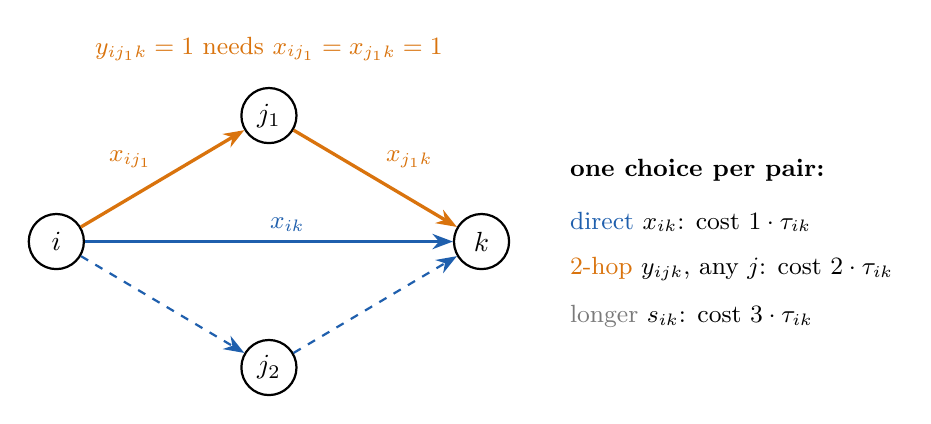
\begin{tikzpicture}
  \node[nd] (i) at (0,0) {$i$};
  \node[nd] (k) at (5.4,0) {$k$};
  \node[nd] (j1) at (2.7,1.6) {$j_1$};
  \node[nd] (j2) at (2.7,-1.6) {$j_2$};
  \draw[ar] (i) -- node[above,pos=.55,font=\small,arc]{$x_{ik}$} (k);
  \draw[pa] (i) -- node[above left,font=\small]{$x_{ij_1}$} (j1);
  \draw[pa] (j1) -- node[above right,font=\small]{$x_{j_1k}$} (k);
  \draw[ar,dashed] (i) -- (j2);
  \draw[ar,dashed] (j2) -- (k);
  \node[path,font=\small] at (2.7,2.45) {$y_{ij_1k}=1$ needs $x_{ij_1}=x_{j_1k}=1$};
  \node[font=\small,anchor=west] at (6.4,0.9) {\textbf{one choice per pair:}};
  \node[font=\small,anchor=west] at (6.4,0.25) {\textcolor{arc}{direct} $x_{ik}$: cost $1\cdot\T_{ik}$};
  \node[font=\small,anchor=west] at (6.4,-0.35) {\textcolor{path}{2-hop} $y_{ijk}$, any $j$: cost $2\cdot\T_{ik}$};
  \node[font=\small,anchor=west] at (6.4,-0.95) {\textcolor{slack}{longer} $s_{ik}$: cost $3\cdot\T_{ik}$};
\end{tikzpicture}
\caption{Each pair with demand is served by the direct arc, by one 2-hop path, or by the
``$\ge3$ hops'' slack. A path variable can be 1 only if both of its arcs are built.}
\end{figure}

%===========================================================================
\section{Strict model (\texttt{build\_path\_qubo})}
\begin{align}
\min\quad & \textstyle\sum_{(i,k)\in\Pairs} \T_{ik}\big(1\cdot x_{ik} + 2\sum_{j} y_{ijk} + 3\, s_{ik}\big)
  &&\text{total flow, 1/2/3 hops}\\
\text{s.t.}\quad
& \textstyle\sum_j x_{ij}=2,\ \ \sum_j x_{ji}=2 && \text{degrees, every node}\\
& x_{ik}+\textstyle\sum_j y_{ijk}+s_{ik}=1 && \text{one choice, every pair}\label{eq:onehot}\\
& y_{ijk}\le x_{ij},\quad y_{ijk}\le x_{jk} && \text{paths only on built arcs}
\end{align}
In QUBO form each equality becomes $\lambda(\cdot)^2$ and each $y\le x$ becomes
$\lambda\,y(1-x)$, where $\lambda$ is the \emph{penalty weight}. For a fixed $x$, the best
path choice gives
$H_2(x)=\sum_{(i,k)\in\Pairs}\T_{ik}\min\{d_{ik}(x),3\}$: total flow with hops capped at~3.

\paragraph{Penalty weight.} Leaving \eqref{eq:onehot} at all zeros costs $\lambda$ but saves up to
$3\T_{ik}\le 3$, so $\lambda>3$ is required. With $\lambda=1$ the sampler ``cheated''.
\paragraph{3-hop extension.} Variables $y_{ijlk}$ (cost 3, slack 4) keep every penalty
quadratic; only the variable count grows.

\section{Soft model and sizes}
The soft model drops the slack and replaces the one-hot equality by pairwise ``at most one''
penalties, each scaled by the pair's demand ($c\ge 1$):
\begin{multline*}
E=\sum_{\Pairs}\T_{ik}\Big[-2x_{ik}-\sum_j y_{ijk}
 + c\sum_j y_{ijk}\big((1-x_{ij})+(1-x_{jk})+x_{ik}\big)
 + c\sum_{j<j'} y_{ijk}y_{ij'k}\Big]\\ + \lambda\cdot(\text{degree penalties}).
\end{multline*}
For $c\ge1$ and any valid $x$: $\min_y E = H_2(x)-3\sum\T_{ik}$, the same objective.
\begin{center}
\begin{tabular}{@{}lrrrrr@{}}
\toprule
instance & $|\Pairs|$ & arcs only & strict 2-hop & soft 2-hop & strict 3-hop\\
\midrule
\texttt{network05} & 13 & 20 & 72 & 59 & 150\\
\texttt{network12} & 88 & 132 & 1\,100 & 1\,012 & 9\,020\\
\texttt{network24} & 350 & 552 & 8\,602 & 8\,252 & 170\,302\\
\bottomrule
\end{tabular}
\end{center}

%===========================================================================
\section{What the path variables bought, and what they cost}
\subsection*{(a) The energy ranks topologies much more like the LP}
Spearman $\rho$ between each surrogate's best-case energy and the LP score. ``Near'' = 300
topologies 1--6 random 2-exchanges from the best known; ``random'' = 300 random valid ones.

\begin{figure}[h]
\centering
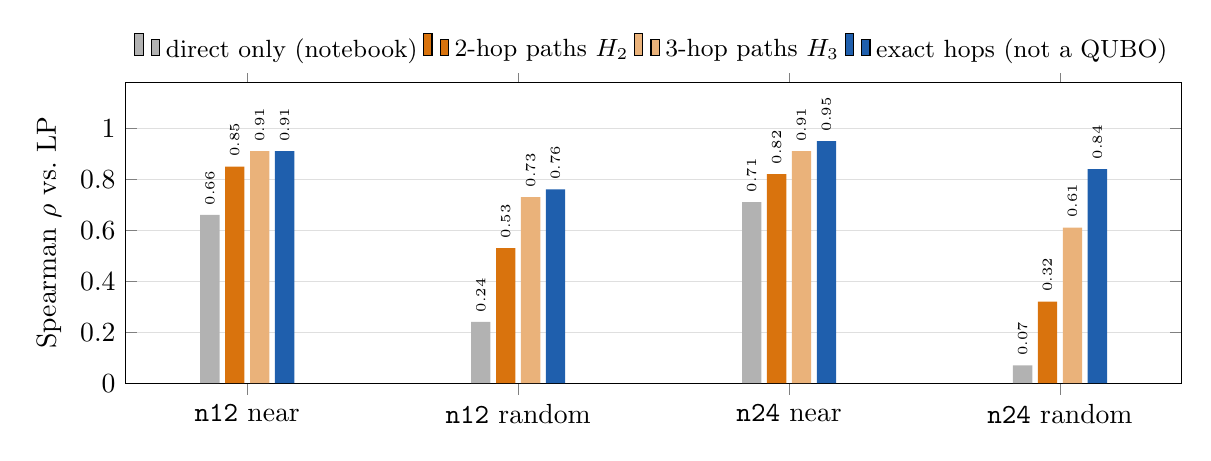
\begin{tikzpicture}
\begin{axis}[
  ybar, bar width=7pt, width=15cm, height=5.4cm,
  ymin=0, ymax=1.18, ytick={0,0.2,...,1}, ylabel={Spearman $\rho$ vs.\ LP},
  point meta=explicit symbolic,
  symbolic x coords={n12 near,n12 rand,n24 near,n24 rand},
  xtick=data, xticklabels={\texttt{n12} near,\texttt{n12} random,\texttt{n24} near,\texttt{n24} random},
  legend style={at={(0.5,1.03)},anchor=south,legend columns=-1,font=\small,draw=none},
  ymajorgrids, grid style={gray!25}, enlarge x limits=0.15,
  nodes near coords, every node near coord/.append style={font=\tiny,rotate=90,anchor=west},
]
\addplot[fill=gray!60,draw=none] coordinates {(n12 near,0.66)[0.66] (n12 rand,0.24)[0.24] (n24 near,0.71)[0.71] (n24 rand,0.07)[0.07]};
\addplot[fill=path,draw=none] coordinates {(n12 near,0.85)[0.85] (n12 rand,0.53)[0.53] (n24 near,0.82)[0.82] (n24 rand,0.32)[0.32]};
\addplot[fill=path!55,draw=none] coordinates {(n12 near,0.91)[0.91] (n12 rand,0.73)[0.73] (n24 near,0.91)[0.91] (n24 rand,0.61)[0.61]};
\addplot[fill=arc,draw=none] coordinates {(n12 near,0.91)[0.91] (n12 rand,0.76)[0.76] (n24 near,0.95)[0.95] (n24 rand,0.84)[0.84]};
\legend{direct only (notebook), 2-hop paths $H_2$, 3-hop paths $H_3$, exact hops (not a QUBO)}
\end{axis}
\end{tikzpicture}
\caption{Path variables raise the correlation with the true score sharply. On
\texttt{network05} every variant gives $\rho=0.43$.}
\end{figure}

\subsection*{(b) \dots but no sampler could minimise those QUBOs (\texttt{network12}, BKV 276\,474)}
\begin{center}\small
\begin{tabular}{@{}llrrr@{}}
\toprule
QUBO & sampler & valid samples & LP best & gap vs BKV\\
\midrule
direct only (132 vars) & SA & all & 314\,500 & $+13.8\%$\\
direct only & partitioned QAOA, GPU & 1/100 & 313\,778 & $+13.5\%$\\
direct only & PCE, polynomial encoding, GPU & 0/100 & 313\,778 & $+13.5\%$\\
strict 2-hop, $\lambda=4\ldots6$ & SA, 2k--20k sweeps & 38--50/50 & 319\,410 & $+15.5\%$\\
soft 2-hop & SA / tabu & 26--50/50 & 324\,112 & $+17.2\%$\\
soft 2-hop & PCE, dense encoding, GPU & 0/100 & 321\,500 & $+16.3\%$\\
soft 2-hop & partitioned QAOA, GPU & 0/100 & 355\,125 & $+28.4\%$\\
soft 2-hop & partitioned PCE, GPU & 13/100 & 407\,500 & $+47.4\%$\\
strict 2-hop & partitioned QAOA, GPU & 0/100 & 425\,334 & $+53.8\%$\\
\bottomrule
\end{tabular}
\end{center}
QUBO sizes: direct 132, soft 2-hop 1\,012, strict 2-hop 1\,100 variables. The last row alone cost 36 Qoro credits. Every result is repaired to a valid topology before LP scoring. For the strict model, SA's
best energy ($67.8$--$70.8$) stayed above that of a known good topology ($62.8$), even with
10$\times$ more sweeps: the \emph{energy function is right, the samplers cannot reach its
minimum}. Partitioning cuts through the degree constraints, so its samples are almost never
valid.

%===========================================================================
\section{The bottleneck: barriers between valid topologies}
On \texttt{network12} only about $5\cdot10^{-25}$ of all arc bitstrings are valid. Two
valid topologies differ in at least 4 bits, because the smallest legal move is the
\emph{2-exchange} $(a\!\to\!b),(c\!\to\!d)\Rightarrow(a\!\to\!d),(c\!\to\!b)$. Walking it one
bit at a time, with degree penalty $\lambda(\deg-2)^2$:
\begin{center}
\begin{tabular}{@{}lll@{}}
\toprule
step & broken degrees & penalty\\
\midrule
start & -- & 0\\
remove $a\to b$ & out($a$)=1, in($b$)=1 & $2\lambda$\\
add $a\to d$ & in($b$)=1, in($d$)=3 & $2\lambda$\\
remove $c\to d$ & in($b$)=1, out($c$)=1 & $2\lambda$\\
add $c\to b$ & -- & 0\\
\bottomrule
\end{tabular}
\end{center}
The barrier ($2\lambda\ge 6$) is much larger than a typical objective change ($0.1$--$1$),
and $\lambda$ cannot be lowered without making violations profitable. Path variables add
more barriers: every path through a changed arc must also switch. The standard X mixer in
QAOA flips bits independently and meets the same wall (1.8\% valid on \texttt{network05}).

\begin{figure}[h]
\centering
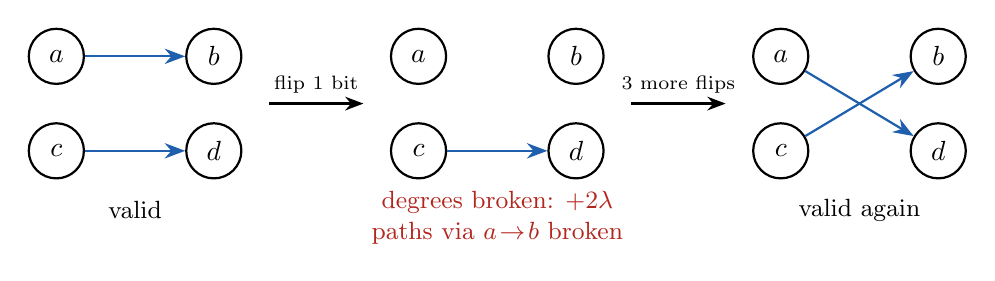
\begin{tikzpicture}
  \begin{scope}
    \node[nd] (a) at (0,1.2) {$a$}; \node[nd] (b) at (2,1.2) {$b$};
    \node[nd] (c) at (0,0) {$c$};   \node[nd] (d) at (2,0) {$d$};
    \draw[ar] (a)--(b); \draw[ar] (c)--(d);
    \node[font=\small] at (1,-0.75) {valid};
  \end{scope}
  \draw[-{Stealth},thick] (2.7,0.6) -- node[above,font=\scriptsize]{flip 1 bit} (3.9,0.6);
  \begin{scope}[xshift=4.6cm]
    \node[nd] (a) at (0,1.2) {$a$}; \node[nd] (b) at (2,1.2) {$b$};
    \node[nd] (c) at (0,0) {$c$};   \node[nd] (d) at (2,0) {$d$};
    \draw[ar] (c)--(d);
    \node[font=\small,bad,align=center] at (1,-0.85) {degrees broken: $+2\lambda$\\paths via $a\!\to\!b$ broken};
  \end{scope}
  \draw[-{Stealth},thick] (7.3,0.6) -- node[above,font=\scriptsize]{3 more flips} (8.5,0.6);
  \begin{scope}[xshift=9.2cm]
    \node[nd] (a) at (0,1.2) {$a$}; \node[nd] (b) at (2,1.2) {$b$};
    \node[nd] (c) at (0,0) {$c$};   \node[nd] (d) at (2,0) {$d$};
    \draw[ar] (a)--(d); \draw[ar] (c)--(b);
    \node[font=\small] at (1,-0.75) {valid again};
  \end{scope}
\end{tikzpicture}
\caption{The smallest legal move needs 4 coordinated arc flips. Every intermediate state
pays a penalty.}
\end{figure}

%===========================================================================
\section{Fix 1: search over 2-exchanges, never single bits}
\texttt{network\_moves.py} replaces Divi's single-bit \texttt{local\_search} with a
\textbf{2-exchange polish}. It ranks all 2-exchange neighbours with a cheap surrogate ($H_2$),
LP-scores the best few, accepts the first improvement and repeats. Every intermediate state
is a valid topology, so no penalty is ever broken. Results on \texttt{network12}, 10 starts,
150 LP evaluations each:
\begin{center}
\begin{tabular}{@{}llrrr@{}}
\toprule
start & neighbour ranking & best & mean & gap vs BKV (best)\\
\midrule
random topology & random & 304\,167 & 313\,322 & $+10.0\%$\\
random topology & $H_2$ & 284\,700 & 292\,359 & $+3.0\%$\\
SA on direct QUBO & $H_2$ & \textbf{282\,819} & 288\,658 & $\mathbf{+2.3\%}$\\
SA on 2-hop QUBO & $H_2$ & 286\,800 & 294\,607 & $+3.7\%$\\
\bottomrule
\end{tabular}
\end{center}
This is the first method within a few percent of BKV. Ranking by $H_2$ is worth about 6\%;
a sampler start adds a little over a random start.

%===========================================================================
\section{Fix 2: an exchange mixer, so QAOA only sees valid topologies}
\subsection{Construction}
One qubit per candidate arc. For each 2-exchange $q=(ab,cd\to ad,cb)$ the mixer adds
\[
  M_q \;=\; \sigma^-_{ab}\,\sigma^-_{cd}\,\sigma^+_{ad}\,\sigma^+_{cb} \;+\; \text{h.c.},
  \qquad \sigma^+=|1\rangle\langle0|,\ \ \sigma^-=|0\rangle\langle1| .
\]
$M_q$ swaps the two arc pairs and acts as zero on any state where the swap is not legal (an
arc already present, or one missing). It expands into 8 mutually commuting 4-qubit Pauli
strings ($X/Y$ with an even number of $Y$). Divi exponentiates term by term, so each
$e^{-i\beta M_q}$ is applied exactly, and each one maps valid topologies to valid
topologies. One mixer layer is the product over all $q$. In/out degrees never change and
the digraph stays simple.

\begin{figure}[h]
\centering
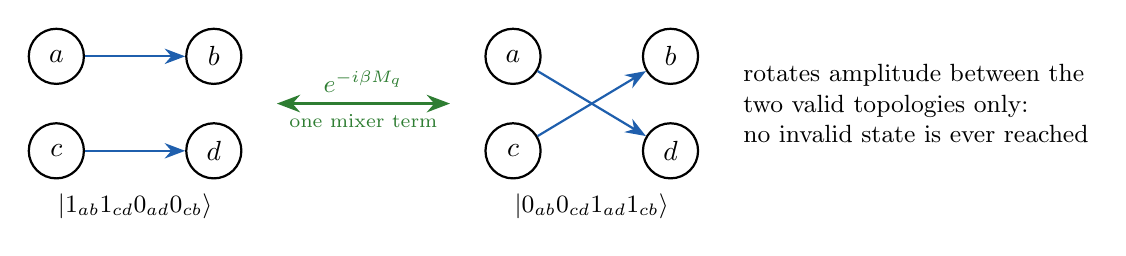
\begin{tikzpicture}
  \begin{scope}
    \node[nd] (a) at (0,1.2) {$a$}; \node[nd] (b) at (2,1.2) {$b$};
    \node[nd] (c) at (0,0) {$c$};   \node[nd] (d) at (2,0) {$d$};
    \draw[ar] (a)--(b); \draw[ar] (c)--(d);
    \node[font=\small] at (1,-0.7) {$|1_{ab}1_{cd}0_{ad}0_{cb}\rangle$};
  \end{scope}
  \draw[{Stealth}-{Stealth},very thick,good] (2.8,0.6) -- node[above,font=\small]{$e^{-i\beta M_q}$}
     node[below,font=\scriptsize,good]{one mixer term} (5.0,0.6);
  \begin{scope}[xshift=5.8cm]
    \node[nd] (a) at (0,1.2) {$a$}; \node[nd] (b) at (2,1.2) {$b$};
    \node[nd] (c) at (0,0) {$c$};   \node[nd] (d) at (2,0) {$d$};
    \draw[ar] (a)--(d); \draw[ar] (c)--(b);
    \node[font=\small] at (1,-0.7) {$|0_{ab}0_{cd}1_{ad}1_{cb}\rangle$};
  \end{scope}
  \node[font=\small,align=left,anchor=west] at (8.6,0.6)
    {rotates amplitude between the\\two valid topologies only:\\no invalid state is ever reached};
\end{tikzpicture}
\caption{The exchange mixer turns a 2-exchange into a single quantum step, so the
penalty barriers of Section~6 are gone.}
\end{figure}

\subsection{Cost without penalties or path variables}
Because every state is valid, the cost Hamiltonian needs no penalty terms. $H_2$ can be
written \emph{exactly} on valid topologies as a degree-4 HUBO in the arc bits (Divi
supports HUBO natively). With $p_j = x_{ij}x_{jk}$:
\[
  H_2 \;=\; \sum_{(i,k)\in\Pairs}\T_{ik}\Big[\,3 - 2x_{ik} - \sum_j p_j + \sum_{j<j'} p_j p_{j'} + x_{ik}\sum_j p_j\Big].
\]
This is exact because node $i$ has only 2 out-arcs: at most two 2-hop paths exist, and at
most one if $x_{ik}=1$, so inclusion--exclusion stops at pairs.

\paragraph{Verified exactly} (local statevector): the HUBO equals $H_2$ on all 216 valid
\texttt{network05} topologies (max error $5\cdot10^{-15}$, 131 terms). After two mixer
layers $P(\text{valid})=1.000000000000$ for $n=4$ (12 qubits) and $n=5$ (20 qubits), and one
starting topology reaches all 9 and all 216 valid topologies respectively.

\subsection{Results on \texttt{network05} (proven optimum 65\,500)}
Exchange-mixer QAOA on the full problem (20 qubits, Qoro GPU), started from a mediocre
random topology (LP 83\,000, rank 107/216):
\begin{center}
\begin{tabular}{@{}lrrrr@{}}
\toprule
layers & $P$(valid) & $P$(LP optimum) & distinct samples & best sampled\\
\midrule
1 & 100\% & 0\% & 85 & 69\,334 \ ($+5.9\%$)\\
2 & 100\% & 0\% & 145 & 68\,000 \ ($+3.8\%$)\\
3 & 100\% & 0.020\% & 161 & \textbf{65\,500} \ (optimal)\\
\midrule
\multicolumn{5}{@{}l}{notebook X mixer + penalties, 2 layers: $P$(valid) 1.8\%, $P$(LP optimum) 0.005\%}\\
\bottomrule
\end{tabular}
\end{center}

\paragraph{Is it reliable?} Pipeline: random start $\to$ exchange-mixer QAOA $\to$ LP-score
the top~10 samples $\to$ 2-exchange polish (20 LP evaluations). Baseline: polish only, same
start, same 30 LP evaluations. Five random starts each:
\begin{center}\small
\begin{tabular}{@{}llccc@{}}
\toprule
layers & candidate selection & in QAOA top 10 & pipeline & polish only\\
\midrule
3 & by sample probability & 2/5 & 3/5 & 3/5\\
3 & by $H_2$ energy & 3/5 & 3/5 & 3/5\\
4 & by sample probability & \multicolumn{3}{c}{\pending\ (so far 2/4 and 2/4)}\\
3, 4 & by energy, COBYLA optimiser & \multicolumn{3}{c}{\pending}\\
\bottomrule
\end{tabular}
\end{center}
\textbf{Diagnosis.} The cost is right: the LP optimum \emph{is} the ground state of $H_2$
(rank 1 of 216). QAOA does not concentrate on it enough: $P$(ground state) was 0--7.8\%,
mean 2.7\%. The polish then gets stuck, because \texttt{network05} has 15 local optima under
2-exchange (68\,000 and 69\,334 trap several starts). Next levers: a stronger angle optimiser
(COBYLA, running), more layers, and more samples.

\subsection{Scaling up}
\begin{itemize}
\item \textbf{\texttt{network06}} (30 qubits, statevector) and \textbf{\texttt{network07}}
  (42 qubits): same pipeline. The 42-qubit statevector job failed on the GPU node, and a
  rerun with an approximate tensor-network simulator (MPS, bond dimension 128) is
  \pending.
\item \textbf{\texttt{network12}} (132 qubits, too many to simulate): the same mixer and
  cost run inside a \emph{quantum local search}. Each step frees 4 arcs; QAOA works on the
  candidate arcs between their tails and heads (at most 16 qubits); fixed arcs are
  substituted into the HUBO; the LP scores the top 3 proposals. All proposers see the same
  freed arcs and the same LP budget:
\end{itemize}
\begin{center}\small
\begin{tabular}{@{}lrrr@{}}
\toprule
proposer (15 steps, $\approx$45 LP evals) & seed 0 & seed 1 & best vs BKV\\
\midrule
random & 336\,334 & 346\,728 & $+21.7\%$\\
classical ($H_2$-ranked enumeration) & 336\,462 & 332\,905 & $+20.4\%$\\
\textbf{QAOA, exchange mixer} & \textbf{324\,834} & \textbf{329\,600} & $+17.5\%$\\
\midrule
\multicolumn{4}{@{}l}{40 steps + 150-eval polish: random 307\,417 ($+11.2\%$), classical 291\,667 ($+5.5\%$), QAOA \pending}\\
\bottomrule
\end{tabular}
\end{center}
$P$(valid) was exactly 1 at every step, and QAOA won on both seeds. The runs are short and
still far from BKV; the 40-step run will show whether the advantage survives convergence.

%===========================================================================
\section{Routing heavy flows through quiet nodes}
\textbf{Idea:} a node $j$ whose own traffic is small ($S_j$ sent, $R_j$ received) has spare
capacity on its links, so transit traffic should prefer it. Let $\mathrm{tr}_j(x)$ be the
transit through $j$ under even splitting over shortest paths. The out-links of $j$ carry
$S_j+\mathrm{tr}_j$ and its in-links $R_j+\mathrm{tr}_j$, two links each, so
$z^\star\ge \max_j \max(S_j,R_j)/2 + \mathrm{tr}_j/2$. We tested three forms:
\begin{itemize}
\item \textbf{linear reward:} total flow $+\ \beta\sum_j w_j\,\mathrm{tr}_j$, with $w_j=(S_j+R_j)/\max$;
\item \textbf{node max:} $\max_j \max(S_j+\mathrm{tr}_j,\ R_j+\mathrm{tr}_j)/2$;
\item \textbf{node L2:} $\sum_j (S_j+\mathrm{tr}_j)^2+(R_j+\mathrm{tr}_j)^2$.
\end{itemize}
\begin{center}
\begin{tabular}{@{}lrrrrr@{}}
\toprule
& \multicolumn{4}{c}{Spearman $\rho$ vs LP} & \texttt{n12}: optimum + polish\\
surrogate & n12 near & n12 rand & n24 near & n24 rand & best (gap vs BKV)\\
\midrule
total flow & 0.83 & 0.71 & 0.93 & 0.81 & 290\,834 ($+5.2\%$)\\
linear reward, $\beta=0.25\ldots2$ & 0.83 & 0.71--0.72 & 0.93 & 0.81 & 283\,334 ($+2.5\%$)\\
node max & 0.81 & 0.76 & 0.89 & 0.72 & 286\,834 ($+3.7\%$)\\
\textbf{node L2} & \textbf{0.85} & \textbf{0.76} & \textbf{0.95} & \textbf{0.85} & 284\,231 ($+2.8\%$)\\
\bottomrule
\end{tabular}
\end{center}
\textbf{Why the linear form does nothing:} $\sum_j w_j\,\mathrm{tr}_j$ is close to (average
$w$)$\times$(total transit), which total flow already counts. \textbf{Why the squared form
works:} its marginal cost for sending more transit through $j$ is $2(S_j+\mathrm{tr}_j)$,
so it penalises busy nodes \emph{and} nodes that already carry a lot of transit. That is
the idea made load-aware. Node L2 has the best surrogate optimum before polishing (294\,236
vs 296\,800 for total flow); after polishing all surrogates land within
283--292k, which 3 restarts cannot separate.

%===========================================================================
\section{Where we stand (\texttt{network12}, BKV 276\,474)}
\begin{center}
\begin{tabular}{@{}lrr@{}}
\toprule
method & best & gap vs BKV\\
\midrule
notebook SA on direct QUBO & 309\,750 & $+12.0\%$\\
any QUBO sampler alone (SA, tabu, partitioned QAOA, PCE) & 313\,778 & $+13.5\%$\\
quantum local search, 15 steps & 324\,834 & $+17.5\%$\\
2-exchange polish, random start & 284\,700 & $+3.0\%$\\
\textbf{SA on direct QUBO + 2-exchange polish} & \textbf{282\,819} & $\mathbf{+2.3\%}$\\
\bottomrule
\end{tabular}
\end{center}

\section{Next steps}
\begin{enumerate}
\item \textbf{Make \texttt{network05} reliable:} raise $P$(ground state) with a stronger
  angle optimiser, more layers and more shots; escape 2-exchange local optima with larger
  moves (3-exchanges) or restarts.
\item \textbf{Scale:} \texttt{network06}/\texttt{07} with the full-problem mixer (MPS for
  wide circuits); \texttt{network12}+ with the quantum local search run to convergence
  and polished, reported against BKV.
\item \textbf{Better cost:} put node L2 into the HUBO (only the terms touched by freed arcs).
\item \textbf{Parked:} PCE and partitioned QAOA break the degree constraints (0--15\% valid
  samples); revisit with constraint-aware partitions or valid-repair decoding.
\end{enumerate}

\vfill
\noindent\footnotesize Code: \texttt{network\_hopqubo.py}, \texttt{network\_hopqubo\_divi.py},
\texttt{network\_moves.py}, \texttt{network\_mixer.py}. Logs: \texttt{runs/hopqubo\_*},
\texttt{runs/moves\_*}, \texttt{runs/mixer\_*}. Cloud runs on Qoro \texttt{qoro\_gpu}.
\end{document}
